\documentclass[]{LASPreport}


\newcommand{\SubSystem}{ADCS}
\newcommand{\SERnumber}{Thruster Unit Test}
\newcommand{\subject}{Unit Test Results for Thruster Simulation Model}
\newcommand{\status}{Initial Test Results}
\newcommand{\preparer}{S. Piggott}
\newcommand{\summary}{
   This is a report documenting the results of the thruster model unit test created for 
   the AVS Basilisk Simulation as part of the EMM project. }


\usepackage[usenames,dvipsnames]{xcolor}
\usepackage{hyperref}

\begin{document}


\makeCover


%
%	enter the revision documentation here
%	to add more lines, copy the table entry and the \hline, and paste after the current entry.
%
\pagestyle{empty}
{\renewcommand{\arraystretch}{2}
\noindent
\begin{longtable}{|p{0.5in}|p{4.5in}|p{1.14in}|}
\hline
{\bfseries Rev}: & {\bfseries Change Description} & {\bfseries By} \\
\hline
Draft & Initial Revision & S. Piggott \\
\hline

\end{longtable}
}

\newpage
\setcounter{page}{1}
\pagestyle{fancy}

\tableofcontents
~\\ \hrule ~\\

%\begin{figure}[htb]
%	\centerline{
%	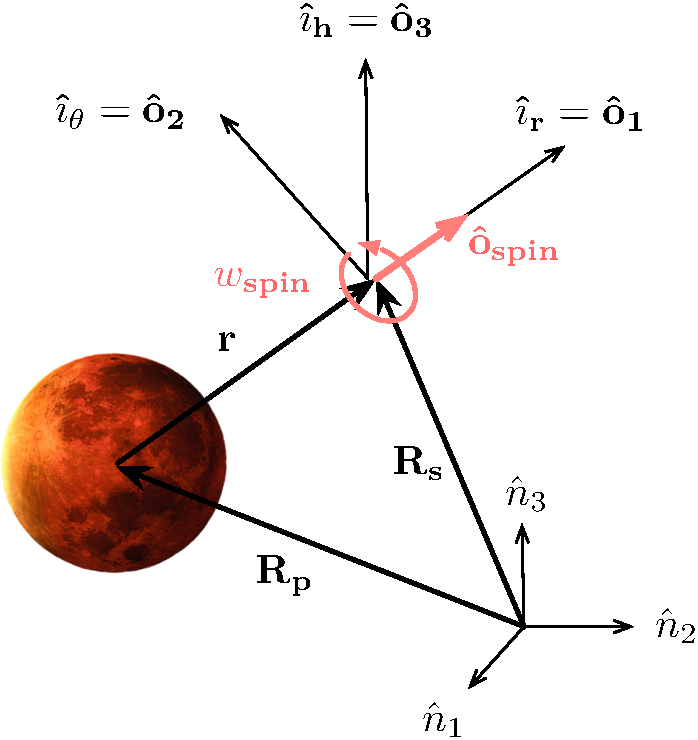
\includegraphics[]{Figures/Fig1}
%	}
%	\caption{Sample Figure Inclusion.}
%	\label{fig:Fig1}
%\end{figure}

\section{Introduction}
The Thruster model in the AVS Basilisk simulation is used to emulate the effect 
of a vehicle's thrusters on the overall system.  Its primary use is to generate 
realistic forces/torques on the vehicle structure and body.  This is 
accomplished by apply a force at a specified location/direction in the body and 
using the current vehicle center of mass to calculate the resultant torque.  
Each individual thruster in a given model has its own ramp-up/ramp-down profile 
specified as part of its initialization data and it follows those profiles during 
start-up and shutdown.

The thruster model also contains a mechanism that is used to change the current 
vehicle mass properties as the thruster fires propellant overboard.  This model 
uses the thruster ISP (specific impulse, also specified with configuration data) 
to calculate how much mass is being removed during a given thruster firing and 
decrements the mass properties included in the thruster linearly as a function 
of mass.  

The model can be configured according to the user's wishes, but the following 
rules of thumb should probably be respected unless you are incredibly confident 
in your own smartness.
\begin{enumerate}
\item{The internal simulation dynamics step time should be less than or equal 
     to the thruster ramp-up/ramp-down time steps}
\item{The internal simulation dynamics step time should be less than or equal to 
     the desired thruster discretization level}
\item{The internal simulation dynamics step time should be less than one-tenth 
    of the expected minimum allowable thruster firing duration}
\end{enumerate}


\section{Test Design}
The unit test for the thruster\_dynamics module is located in:\\

\noindent
{\tt SimCode/dynamics/Thrusters/UnitTest/ThrusterDynamicsUnitTest.py} \\
\\

\noindent This unit test is designed to functionally test the simulation model 
outputs as well as get complete code path coverage.  The test design is broken 
up into several parts:\\
\begin{enumerate}
\item{Thruster Force Orientation: The output forces/torques from the simulation 
  are checked to ensure that their values/directions are correct per the 
  simulation inputs.}
\item{Instantaneous On/Off Factor: The thrusters are fired with an 
  instantaneous ramp to ensure that the firing is correct depending on the 
  simulation dynamics rate.  This includes propellant depletion.}
\item{Short Instantaneous Firing: A "short" firing that still respects the 
  rules of thumb above is fired to ensure that it is still correct enough.}
\item{Ramp On/Ramp Off Firing: A set of ramps are set for the thruster to ensure 
  that the ramp configurationis respected during a ramped firing.}
\item{Short firing: A thruster is fired for less than the amount of time it 
   takes to reach the end of its ramp.}
\item{Cutoff firing: A thruster is commanded off (zero firing time) in the middle 
   of its ramp up to ensure that it correctly cuts off the current firing}
\item{Ramp down firing: A thruster is fired during the middle of its ramp down 
   to ensure that it picks up at that point in its ramp-up curve and reaches 
   steady state correctly.}
\item{Propellant Consumption: The propellant consumption for the duration of the 
    test is checked at each time step to ensure that it is correct for each 
    point in time in the test.}
\end{enumerate}


\section{Test Results}


\begin{enumerate}
\item{Thruster Force Orientation: The thruster is pointed with a 30 degree cant 
    off of the x-axis such that it fires with the sine of 30 in the y-axis 
    and the cosine of 30 in the x-axis.  Then the structure to body rotation 
    is configured with a 180 degree yaw such that the values in the axes are 
    negated in the body frame. Figure \ref{fig:force_vec_fig} shows a plot of 
    this behavior for the thruster unit test.
    \begin{figure}[htb]
            \centerline{
            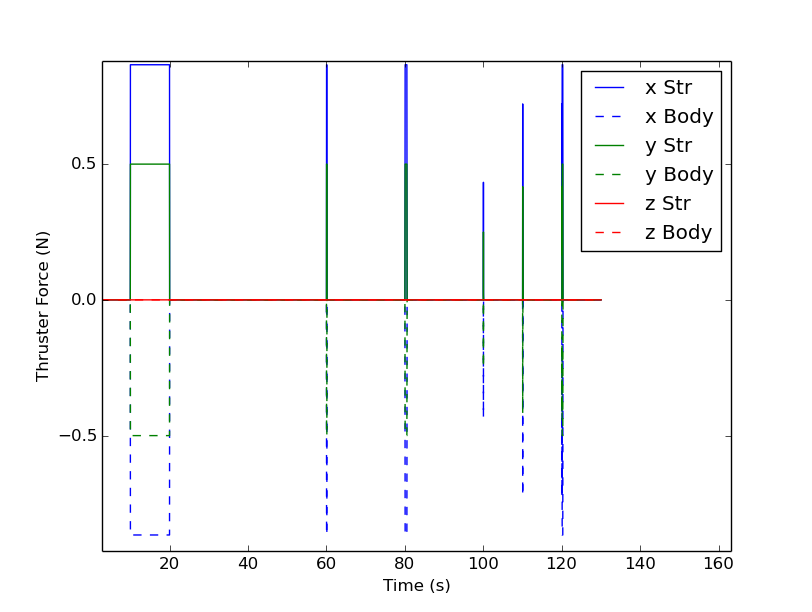
\includegraphics[scale=0.5]{Figures/thrusterForceData}
            }
            \caption{Structural and Body Forces for Thruster Unit Test}
            \label{fig:force_vec_fig}
    \end{figure}
    As this figure shows, the desired behavior is captured exactly for each 
    firing in the test.  \textcolor{ForestGreen}{Test successful.}
}
\item{Instantaneous On/Off Factor:  The main driving force for the overall 
    thrust coming out of a thruster in the model is the instantaneous thrust 
    factor.  This parameter will be the primary check for the rest of the test. 
    A single firing was commanded with a duration of 10 seconds.  No thruster 
    ramp was used for either the ramp-up or ramp-down.  The expected total 
    duration for the thruster firing was 10.0 seconds.  Figure 
    \ref{fig:first_inst_fir} shows a plot of the thrust factor for this firing.
    \begin{figure}[htb]
            \centerline{
            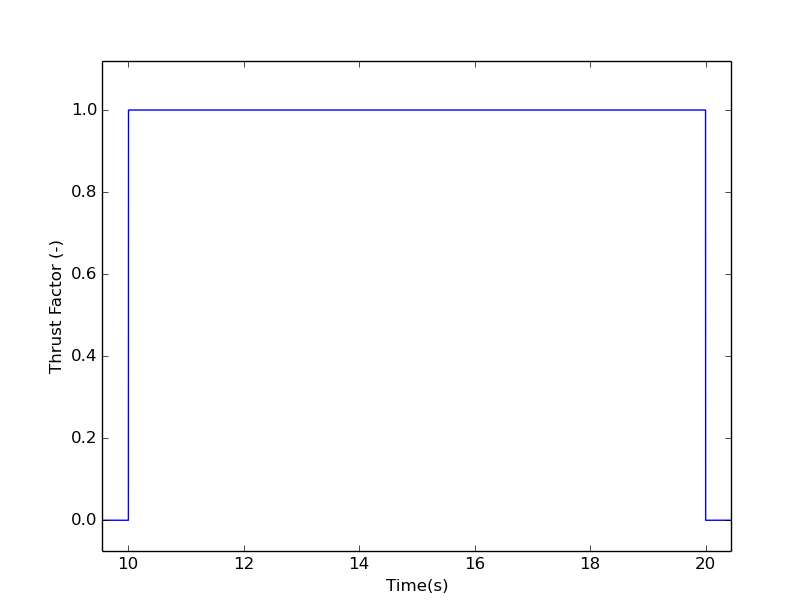
\includegraphics[scale=0.5]{Figures/firstInstantFiring}
            }
            \caption{Thrust factor for 10.0 second firing}
            \label{fig:first_inst_fir}
    \end{figure}
    As this plot shows, the thruster does jump to the appropriate firing level 
    as soon as it turns on.  There are two funnies that need to be verified in 
    a different test.  The thrust factor is designed to be driven during the 
    derivative step of dynamics with a multi-step integrator.  In order to test 
    this single model, this dynamics effect was emulated in the test driver.  
    However this indicates that the thruster terminates one dynamics cycle prior 
    to 10.0 seconds and reflects this effect regardless of the dynamics step 
    used.  This is nominal because of the dynamics emulation but an integrated 
    test does need to be performed to verify that the integrated impulse is 
    correct for a single firing.  \textcolor{ForestGreen}{Test successful.}
}
\item{Short Instantaneous Firing: Similar to the previous test, a non-ramped 
    firing was commanded with a shorter duration of 0.1 seconds to ensure that 
    the firing shows the same overall behavior as a long-duration firing.  
    Figure \ref{fig:second_inst_fir} shows the plot for this firing.

    \begin{figure}[htb]
            \centerline{
            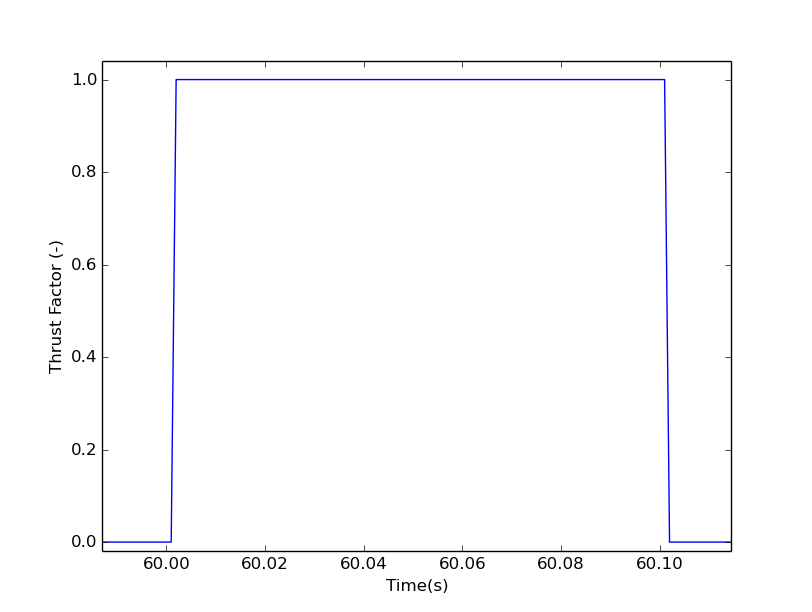
\includegraphics[scale=0.5]{Figures/secondInstantFiring}
            }
            \caption{Thrust factor for 0.1 second firing}
            \label{fig:second_inst_fir}
    \end{figure}
    As this figure shows, the short firing behaves exactly as expected with the 
    same character as the results shown in the previous test.
    \textcolor{ForestGreen}{Test successful.}
}
\item{Ramp On/Ramp Off Firing:  This test was performed with a thruster 
    ramp model added for both the startup and the shutdown of the thruster.  
    Both the startup and shutdown ramps were setup such that they ramp linearly 
    and take 30 ms to reach steady-state thrust.  Figure \ref{fig:first_ramp_fir} 
    shows the thrust factor to this ramped firing.
    \begin{figure}[htb]
            \centerline{
            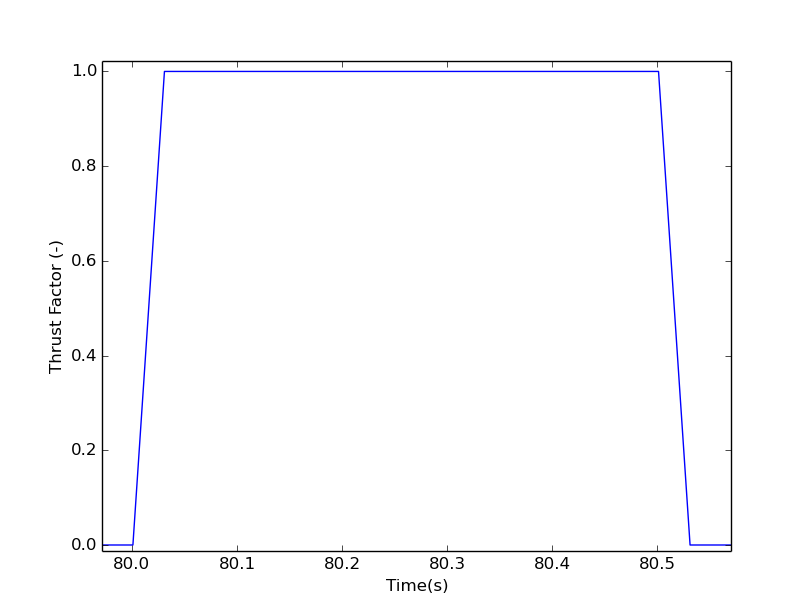
\includegraphics[scale=0.5]{Figures/firstRampFiring}
            }
            \caption{Thrust factor for 0.5 second ramped firing}
            \label{fig:first_ramp_fir}
    \end{figure}
    As this figure shows, both the startup and shutdown transients ramped 
    according to the expected profile and both were checked to ensure that 
    they took the expected 30 ms to ramp. 
    \textcolor{ForestGreen}{Test successful.}
}
\item{Short firing:  This test was performed with a short firing that did not 
    reach the steady-state thrust level for the thruster.  It was commanded on 
    for a duration of 15 ms such that it should only get to a 50\% thrust level 
    with the total firing duration being 30 ms from start to shutdown.  Figure 
    \ref{fig:short_ramp_fir} shows the results of this test.
    \begin{figure}[htb]
            \centerline{
            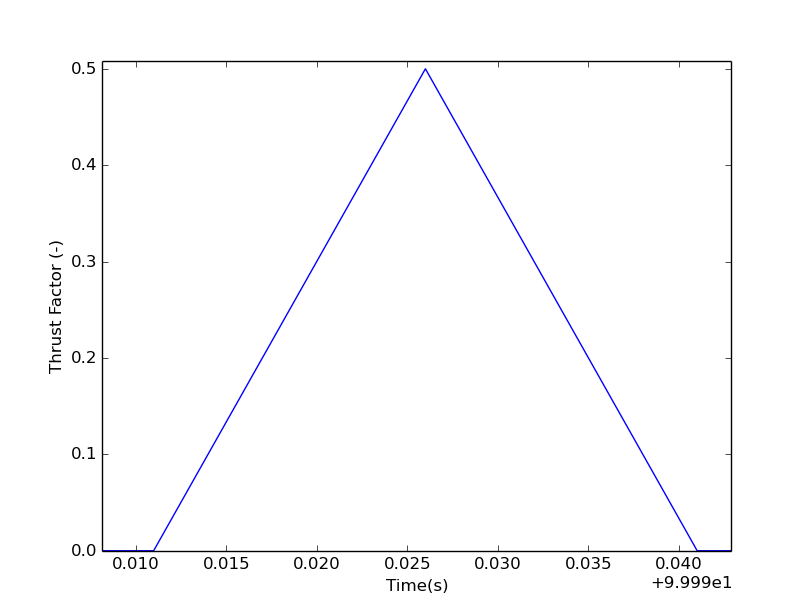
\includegraphics[scale=0.5]{Figures/shortRampFiring}
            }
            \caption{Thrust factor for 0.015 second ramped firing}
            \label{fig:short_ramp_fir}
    \end{figure}
    As the figure shows, the test performed exactly as expected.  The thrust 
    factor ramped linearly to 50\% and then down to zero in exactly 30 ms.  
    	\textcolor{ForestGreen}{Test successful.}
}
\item{Cutoff firing:  This test contained two commanded firings.  The first 
    command was set for 0.5 seconds and the simulation was then advanced for 
    0.02 seconds.  Then a new command was injected to the system with a duration 
    of 0.005 seconds.  The intent in this case is to end up with a net command 
    that looks like it was set for 0.025 seconds to ensure that the new command 
    was followed and correctly overrode the previous command.  Figure 
    \ref{fig:cutoff_ramp_fir} shows the results from this test.
    \begin{figure}[htb]
            \centerline{
            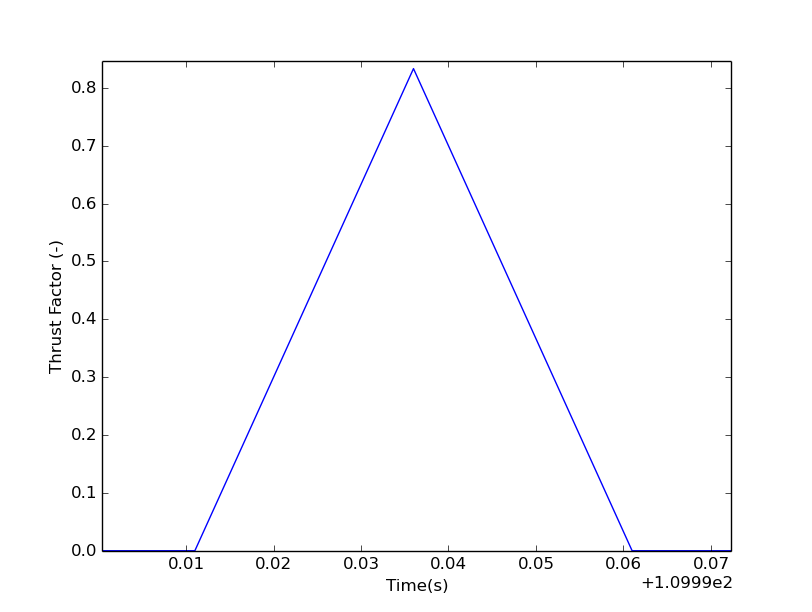
\includegraphics[scale=0.5]{Figures/cutoffRampFiring}
            }
            \caption{Thrust factor for cutoff ramped firing}
            \label{fig:cutoff_ramp_fir}
    \end{figure}
    As the figure shows, the expected behavior is observed exactly.  The thruster 
    ramps to 0.8333 in thrust factor with the total firing duration being 0.05 
    seconds.  	\textcolor{ForestGreen}{Test successful.}
}
\item{Ramp down firing:  This test contained two firings again.  The first 
    command was set for 0.025 seconds to have the thrust start to ramp down 
    0.025 seconds after init.  Then a second command was sent after 0.04 seconds 
    in the middle of the thruster's ramp-down to ensure that the command picked 
    back up where the thrust was tailing off, ramped up to steady-state, and 
    ramped down after the command (0.2 seconds) was fulfilled.  Figure 
    \ref{fig:middle_ramp_fir} shows the model's thrust for this particular 
    command set.
    \begin{figure}[htb]
            \centerline{
            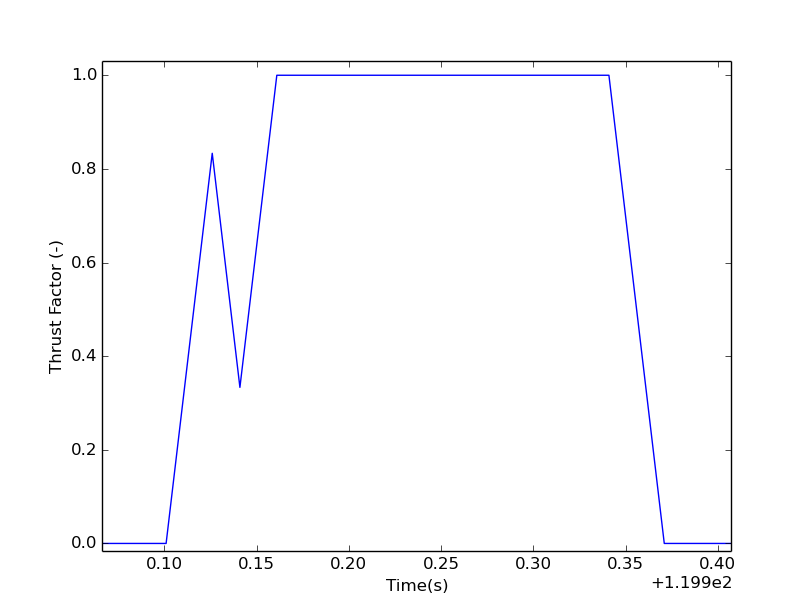
\includegraphics[scale=0.5]{Figures/middleRampFiring}
            }
            \caption{Thrust factor for firing during shutdown}
            \label{fig:middle_ramp_fir}
    \end{figure}
    This test also performed nominally.  The first firing ramped to 0.025 seconds 
    and then began turning off.  Then the second command was picked up and the 
    thrust ramped smoothly until the total duration of 0.2 seconds was reached 
    followed by a ramp down.  The total expected firing for this particular 
    sequence is 0.04 + 0.2 + 0.03 or 0.27 seconds which matches the observed 
    duration exactly.  	\textcolor{ForestGreen}{Test successful.}
}
\item{Propellant Consumption: This test was performed against each firing to 
    ensure that the propellant consumed during the test was correct at each time 
    step.  The propellant consumption was correct to less than 0.1\%.  That is 
    sufficiently accurate compared to other modeling inaccuracies in the model.
    \textcolor{ForestGreen}{Test successful.}
}
\end{enumerate}

\section{Test Coverage}
The method coverage for all of the methods included in the spice\_interface 
module are tabulated in Table~\ref{tab:cov_met}

\begin{table}[htbp]
    \caption{Test Analysis Results}
   \label{tab:cov_met}
        \centering \fontsize{10}{10}\selectfont
   \begin{tabular}{c | r | r | r} % Column formatting, 
      \hline
      Method Name    & Unit Test Coverage (\%) & Runtime Self (\%) & Runtime Children (\%) \\
      \hline
      SelfInit & 100.0 & 0.0 & 0.0 \\
      CrossInit & 100.0 & 0.0 & 0.0 \\
      AddThruster & 100.0 & 0.0 & 0.0 \\
      UpdateState & 100.0 & 0.0 & 0.0 \\
      WriteOutputMessages & 100.0 & 0.0 & 0.0 \\
      ReadInputs & 100.0 & 0.0 & 0.0 \\
      ConfigureThrustRequests & 100.0 & 0.0 & 0.0 \\
      ComputeDynamics & 100.0 & 0.0 & 9.8 \\
      ComputeThrusterFire & 100.0 & 0.0 & 0.0 \\
      ComputeThrusterShut & 100.0 & 0.0 & 0.0 \\
      updateMassProperties & 100.0 & 0.0 & 0.6 \\
      \hline
   \end{tabular}
\end{table}

For all of the methods in the spice\_interface modules, the code coverage 
percentage is 100\% which meets our test requirements.  Additionally, 100\% of 
all code branches in the thruster\_dynamics source code were executed by this 
test.

The test that was run to calculate thruster CPU usage was deliberately selected as 
a stressing case for the thruster model.  The MOI burn was executed 9000 seconds 
after the simulation was initialized and that maneuver takes 2000 seconds, so 
approximately 20\% of the simulation was run with the vehicle under thrust.  
With this stressing case, the ThrusterDynamics model accounted for 10\% of the 
overall processing, which is certainly acceptable at this time.

The main CPU usage of the thruster\_dynamics source code occurs in the 
ComputeDynamics method that is called by the dynamics source.  The 
ThrusterDynamics methods themselves account for very little of the processing 
and it is the vector/matrix manipulation utilities called from the source that 
are the main culprits.  While the thruster model's ComputeDynamics function is 
using 50\% of the dynamics processing, that is only amounting to 10\% of the 
overall simulation processing.  The rest of the architecture in Basilisk should 
allow us to take the processing hit that we are getting from the 
ThrusterDynamics module without issue.

\section{Conclusions}
The thruster\_dynamics module has sufficient fidelity to accomplish the analysis 
that we need to perform for the EMM spacecraft.  All model capabilities were 
tested and analyzed in this document with all observed performance being nominal 
compared to the going-in expectation.  

Every line of source code was successfully tested and the integrated model 
performance was analyzed and is acceptable.  There are small updates that could 
be made to get a slight performance increase if necessary, but the work that 
would be required to get that performance bump does not seem worthwhile at this 
time especially since the vehicle (and all spacecraft) spends so little of its 
time under thrust.

\end{document}
